% File:     spconf.sty          (LaTeX Document style option "spconf")
%
% Usage:    \documentclass{article}
%           \usepackage{spconf}
%
%           Or for LaTeX 2.09:
% Usage:    \documentstyle[...,spconf,...]{article}
%
% Purpose:
%
% Style file for Signal Processing Society Conferences (ICASSP, ICIP).
% Features:
%    - correct page size (175mm x 226mm)
%    - twocolumn format
%    - boldfaced, numbered, and centered section headings
%    - correct subsection and subsubsection headings
%    - use \title{xx} for title, will be typeset all uppercase
%    - use \name{xx} for author name(s) only, will be typeset in italics
%    - use \address{xx} for one address of all authors
%    - use \twoauthors{author1}{address1}{author2}{address2}
%         for two (or more) authors with two separate addresses
%    - note: no need for \author nor \date
%    - optional: can use \thanks{xx} within \name or \twoauthors,
%         asterisk is not printed after name nor in footnote
%    - optional: can use \sthanks{xx} after each name within \name or
%         \twoauthors if different thanks for each author,
%         footnote symbol will appear for each name and footnote
%    - optional: use \ninept to typeset text in 9 pt; default is 10pt.
%
% Example of use for one or more authors at a common address and
%    common support. For distinct support acknowledgments,
%    use \sthanks{xx} after each name.
%
%                 \documentclass{article}
%                 \usepackage{spconf}
%                 \title{Title of the paper}
%                 \name{George P. Burdell and John Q. Professor
%                       \thanks{This work was supported by...}}
%                 \address{Common address, department \\
%                          City, etc \\
%                          optional e-mail address}
%
%                 \begin{document}
%  OPTIONAL -->   \ninept            <-- OPTIONAL, for nine pt only
%                 \maketitle
%                 \begin{abstract}
%                 This is the abstract for my paper.
%                 \end{abstract}
%                         .
%                 Insert text of paper
%                         .
%                 \end{document}
%
% Example of use for two authors at two distinct addresses with only
%    one support acknowledgment. For distinct support acknowledgments,
%    use \sthanks{xx} after each name.
%
%                 \documentclass{article}
%                 \usepackage{spconf}
%                 \title{Title of the paper}
%                 \twoauthors{John Doe
%                       \thanks{This work was supported by...}}
%                            {Doe's address, department \\
%                             City, etc \\
%                             optional e-mail address}
%                            {Judy Smith}
%                            {Smith's address, department \\
%                             City, etc \\
%                             optional e-mail address}
%
%                 \begin{document}
%  OPTIONAL -->   \ninept            <-- OPTIONAL, for nine pt only
%                 \maketitle
%                 \begin{abstract}
%                 This is the abstract for my paper.
%                 \end{abstract}
%                         .
%                 Insert text of paper
%                         .
%                 \end{document}
%
% Preprint Option (Only for preprints, not for submissions!):
%    - can create a preprint titlepage footer by using the
%         "preprint" option with the \usepackage{spconf} command
%    - use \copyrightnotice{\copyright xx} for copyright information
%    - use \toappear{To appear in xx} for publication name
% Example of preprint use:
%
%                 \documentclass{article}
%                 \usepackage[preprint]{spconf}
%                         .
%                 \copyrightnotice{\copyright\ IEEE 2000}
%                 \toappear{To appear in {\it Proc.\ ICASSP2000,
%                    June 05-09, 2000, Istanbul, Turkey}}
%
%
% PLEASE REPORT ANY BUGS
%
% Author:  Stephen Martucci  -- stephen.martucci@ieee.org
%
% Date:    3 May 2000
%
% Updated: Lance Cotton, Ulf-Dietrich Braumann, 11 May 2006
% Change:  Added keywords/Index Terms section
% Change:  Added \emergencystretch=11pt, Lance Cotton, 26-Sept-2007
%
%%%%%%%%%%%%%%%%%%%%%%%%%%%%%%%%%%%%%%%%%%%%%%%%%%%%%%%%%%%%%%%%%%%%%%%%

% These commands change default text fonts to the scalable PostScript
% fonts Times, Helvetica, and Courier. However, they do not change
% the default math fonts. After conversion to PDF, text will look good
% at any scale but math symbols and equations may not.
% If instead you use the PostScript Type 1 implementation of the
% Computer Modern fonts from the American Mathematical Society, which
% will make all fonts (text and math) scalable, comment out the
% following three lines. Those fonts use the same metrics as the Knuth
% Computer Modern fonts and therefore no font redefinition is needed.
\renewcommand{\sfdefault}{phv}
\renewcommand{\rmdefault}{ptm}
\renewcommand{\ttdefault}{pcr}

%\oddsidemargin  -0.31in
%\evensidemargin -0.31in
\oddsidemargin  -6.2truemm
\evensidemargin -6.2truemm

\topmargin 0truept
\headheight 0truept
\headsep 0truept
%\footheight 0truept
%\footskip 0truept
\textheight 229truemm
\textwidth 178truemm

\twocolumn
\columnsep 6truemm
\pagestyle{empty}

\emergencystretch=11pt

\def\ninept{\def\baselinestretch{.95}\let\normalsize\small\normalsize}

\def\maketitle{\par
 \begingroup
 \def\thefootnote{}
 \def\@makefnmark{\hbox
 {$^{\@thefnmark}$\hss}}
 \if@twocolumn
 \twocolumn[\@maketitle]
 \else \newpage
 \global\@topnum\z@ \@maketitle \fi\@thanks
 \endgroup
 \setcounter{footnote}{0}
 \let\maketitle\relax
 \let\@maketitle\relax
 \gdef\thefootnote{\arabic{footnote}}\gdef\@@savethanks{}%
 \gdef\@thanks{}\gdef\@author{}\gdef\@title{}\let\thanks\relax}

\def\@maketitle{\newpage
 \null
 \vskip 2em \begin{center}
 {\large \bf \@title \par} \vskip 1.5em {\large \lineskip .5em
\begin{tabular}[t]{c}\@name \\ \@address
 \end{tabular}\par} \end{center}
 \par
 \vskip 1.5em}

\def\title#1{\gdef\@title{\uppercase{#1}}}
\def\name#1{\gdef\@name{{\em #1}\\}}
\def\address#1{\gdef\@address{#1}}
\gdef\@title{\uppercase{title of paper}}
\gdef\@name{{\em Name of author}\\}
\gdef\@address{Address - Line 1 \\
               Address - Line 2 \\
               Address - Line 3}



\def\twoauthors#1#2#3#4{\gdef\@address{}
   \gdef\@name{\begin{tabular}{@{}c@{}}
        {\em #1} \\ \\
        #2\relax
   \end{tabular}\hskip 1in\begin{tabular}{@{}c@{}}
        {\em #3} \\ \\
        #4\relax
\end{tabular}}}

\def\@sect#1#2#3#4#5#6[#7]#8{
   \refstepcounter{#1}\edef\@svsec{\csname the#1\endcsname.\hskip 0.6em}
       \begingroup \ifnum #2=1\bf\centering
          {\interlinepenalty \@M
             \@svsec\uppercase{#8}\par}\else\ifnum #2=2\bf
          \noindent{\interlinepenalty \@M \@svsec #8\par}\else\it
          \noindent{\interlinepenalty \@M
             \@svsec #8\par}\fi\fi\endgroup
       \csname #1mark\endcsname{#7}\addcontentsline
         {toc}{#1}{\protect\numberline{\csname the#1\endcsname} #7}
     \@tempskipa #5\relax
     \@xsect{\@tempskipa}}

\def\abstract{\begin{center}
{\bf ABSTRACT\vspace{-.5em}\vspace{0pt}}
\end{center}}
\def\endabstract{\par}

% Keyword section, added by Lance Cotton, adapted from IEEEtrans, corrected by Ulf-Dietrich Braumann
\def\keywords{\vspace{.5em}
{\bfseries\textit{Index Terms}---\,\relax%
}}
\def\endkeywords{\par} 

\long\def\@makecaption#1#2{
 \vskip 10pt
 \setbox\@tempboxa\hbox{#1. #2}
 \ifdim \wd\@tempboxa >\hsize #1. #2\par \else \hbox
to\hsize{\hfil\box\@tempboxa\hfil}
 \fi}

\def\fnum@figure{{\bf Fig.\ \thefigure}}
\def\fnum@table{{\bf Table \thetable}}

\flushbottom

%%%% EOF

% Template for ICASSP-2021 paper; to be used with:
%          spconf.sty  - ICASSP/ICIP LaTeX style file, and
%          IEEEbib.bst - IEEE bibliography style file.
% --------------------------------------------------------------------------
\documentclass{article}
\usepackage{spconf,amsmath,graphicx}
\usepackage[tableposition=top]{caption}
\usepackage{multirow}

% Example definitions.
% --------------------
\def\x{{\mathbf x}}
\def\L{{\cal L}}

% Title.
% ------
\title{A METHOD FOR DETECTING CORONARY ARTERY DISEASE USING NOISY ULTRASHORT ELECTROCARDIOGRAM RECORDINGS}
%
% Single address.
% ---------------
\name{Orestis Apostolou$^{\star}$ \qquad Vasileios Charisis$^{\star}$ \qquad Georgios Apostolidis$^{\star}$ \qquad Leontios J. Hadjileontiadis$^{\dagger,\star}$\thanks{This research project was funded by the Abu Dhabi Department of Education and Knowledge (ADEK),
UAE, under the Award for Research Excellence (AARE) 2018, ref. no: 29934 }}
 \address{$^{\dagger}$Department of Electrical \& Computer Eng., Khalifa University, PO Box 127788, UAE\\
 $^{\star}$ Department of Electrical \& Computer Eng., Aristotle University of Thessaloniki, GR-54124, Greece}
%
% For example:
% ------------
%\address{School\\
%	Department\\
%	Address}
%
% Two addresses (uncomment and modify for two-address case).
% ----------------------------------------------------------
%\twoauthors
%  {A. Author-one, B. Author-two\sthanks{Thanks to XYZ agency for funding.}}
%	{School A-B\\
%	Department A-B\\
%	Address A-B}
%  {C. Author-three, D. Author-four\sthanks{The fourth author performed the work
%	while at ...}}
%	{School C-D\\
%	Department C-D\\
%	Address C-D}
%
\begin{document}
%\ninept
%
\maketitle
%
\begin{abstract}
The current study aims at creating an algorithm able to detect Coronary Artery Disease (CAD), using ultrashort (duration of 30 seconds) one-lead ECG recordings. The presented method is designed to allow both electrode and noisy recordings (deriving from a smartwatch) as input. This is achieved by using an autoencoder neural network, which inspects the quality of each recording. The algorithm's core is a Support Vector Machine (SVM) model, which evaluates each patient's recordings and predicts whether they indicate CAD. Using statistics and combining the models mentioned above, a light, reliable, easy to use predicting system is created, suitable for deployment in a mobile application, which uses a smartwatch as its recording tool.
\end{abstract}
%
\begin{keywords}
coronary artery disease, autoencoder, SVM, electrocardiogram, smartwatch
\end{keywords}
%
\section{Introduction}
\label{sec:intro}
During the last decade, there has been an exponential rise in the applications which use Artificial Intelligence (AI). More problems, which seemed unsolvable in the previous century, are now resolved with remarkable effectiveness using AI systems. The capabilities created by utilizing the tool abundance a scientist has in hands are limitless. The results of this scientific flourishing are effortless to spot in everyday life.
%One of the engineering fields, which seems to be in its early stages, is the bioengineering field. The much challenging nature of the medical problems, deriving from the multifactor environment in which they are detected, as well as the uncertainty existing in each independent stage and the objective difficulties in coping with scientific issues, are only a few of the factors to be blamed for the slower evolution of this specific field. Even when new innovative methods of dealing with medical issues arise, people tend to be undemonstrative.%
The current study suggests a diagnostic method for CAD \cite{CAD_article}. CAD is the narrowing or the blockage of the heart arteries caused by the buildup of fat, cholesterol, and other substances, a situation known as atherosclerosis. If not detected timely, it can lead to heart failure or death. In 2015, CAD was responsible for 15.6\% of the total deaths in the year, making it the most common death factor globally.

During the last years, many AI algorithms have been created trying to detect CAD at early stages. Most of them use long-duration ECG recordings (24-hour or 15-minute) as input, and with the aid of either classic machine learning or deep learning methods, they predict the existence of CAD.
Some of those techniques are very effective, approaching the accuracy of 100\% in their predictions. However, those techniques are challenging to use in daily life due to people's limited access to accurate digital ECGs. Even when that access is feasible, it is impractical to utilize this technique for everyday use.

In the current study, we approach the issue from a different perspective. There has been an effort to create a light algorithm that uses ECG recordings of 30 seconds duration, suitable for coping with either noiseless waveforms deriving from electrodes or noisy waveforms coming from smartwatches. Initially, ECGs are separated into R-R intervals, and afterward, each interval is imported into an autoencoder network. The network tries to reconstruct the initial R-R waveform and estimates the current noise level. If this level exceeds a certain threshold, then the waveform is characterized as noisy. After evaluating each R-R interval, it is adjudicated if the 30-second sample contains a significant amount of noise. If so, the waveform is rejected as noisy. If not, it proceeds in the following stages of the procedure. During these stages, feature extraction is executed, which is followed by a Principal Component Analysis. Then, the modified features are imported into an SVM model to be classified as having CAD or not. The last stage of the algorithm is the evaluation of more recordings coming from the same person so that the final result can be more accurate.

Regarding the structure of the current study, the preprocessing algorithm stages are described in Section 2. In Section 3, all details of the SVM model are presented. The statistical methods used for the evaluation are included in Section 4. In Section 5, the method and its individual stages are evaluated. In Section 6, comparisons to other published studies are presented, and Section 7 concludes the paper.
%
\section{PREPROCESSING}
\label{sec:preprocessing}
The preprocessing stages presented here were applied both for the training and testing data of the SVM. This way, objective evaluation of the procedure was ensured.
%
\subsection{Data acquisition}
\label{ssec:data_acquisition}
The data used in the application fall into two categories: data of people having CAD and data of people without CAD. The separation was designed so that the final classification problem would be whether a person has CAD or not. The databases used were MIT-BIH Normal Sinus Rhythm Database \cite{goldberger2000physiobank}, Long Term ST Database \cite{jager2003long}, and the Combined measurement of ECG, Breathing, and Seismocardiograms \cite{garcia2013comparison}. Those three databases contain long-duration ECGs. Therefore the data was separated into samples of 30 seconds. There were available recordings of 56 people with CAD (35 men, 21 women) and 39 healthy people (17 men, 22 women) in total. 

Among the CAD patients, some subjects also had other medical diagnoses. To achieve a total classification focus in CAD detection, we used only samples from people who suffered exclusively from CAD or were completely healthy in the model training procedure. Thus, there were 25 subjects diagnosed with CAD and 18 healthy used for training. The rest of the data was used for testing purposes. 
%
\subsection{R-R intervals separation}
\label{ssec:RR_intervals_separation}
It is widely known that the movement of the heart muscles is periodic, and it can be separated into segments. The most characteristic section in a circadian circle is the R peak, representing the heartbeat. The detection of the R peaks is a critical stage of the preprocessing of the application. The problem of peak detection has been encountered with numerous different approaches and, many times, with exceptional accuracy. 
The current application uses a variation of the classic Pan-Tompkins algorithm \cite{pan_tompkins, sedghamiz2018biosigkit}. This variation is not real-time; hence, it is not restricted to processing causal signals. This property helps the algorithm correct the mispredictions created at the beginning of the waveform caused by the initialization of the filters. Also, it allows the algorithm to rectify other mispredictions as well.

\subsection{Autoencoder}
\label{ssec:autoencoder}
Taking into consideration that the recordings used in the application may originate from smartwatches, they may include significant noise levels. The current application tries to detect recordings containing significant noise levels and reject them so that they do not lead to mispredictions. For that reason, an autoencoder neural network was constructed aimed to detect abnormalities in the R-R samples. This network consists of one encoder and one symmetrical decoder, each one having three hidden layers. The neural network intends to reconstruct the initial R-R sample. Random sample intervals from the healthy dataset were used (some of the non-healthy people display heart episodes that cause non-regular heartbeats) to train the neural network. After completing the network training, all the reconstructions' mean absolute error is calculated by comparing the initial waveform and its reconstruction. If it is found to exceed the selected threshold, the R-R interval is labeled as noisy. This threshold was chosen to be equal to $E\{MAE\} + 2.5 \cdot\sigma\{MAE\}$. Finally, if the percentage of the noisy R-R intervals is greater than 50\%, the whole 30-second sample is being labeled as noisy and gets rejected from the rest of the procedure.
%
\begin{figure}[t!]
    \begin{minipage}[b]{.48\linewidth}
        \centering
        \centerline{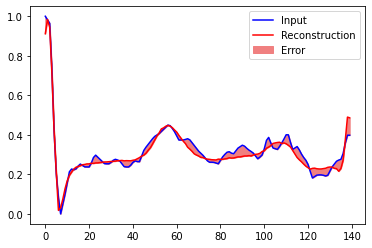
\includegraphics[scale=0.31]{autoenc_good.png}}
        %  \vspace{1.5cm}
        \centerline{(a)}\medskip
    \end{minipage}
%\hfill
    \begin{minipage}[b]{0.48\linewidth}
        \centering
        \centerline{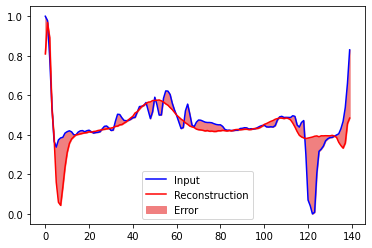
\includegraphics[scale=0.31]{autoenc_bad.png}}
        %  \vspace{1.5cm}
        \centerline{(b)}\medskip
    \end{minipage}
%
\caption{Example of R-R interval reconstruction created by the autoencoder network. (a) Noiseless and (b) Noisy reconstruction.}
\label{fig:res}
%
\end{figure}
%
\subsection{Features extraction}
\label{ssec:features_extraction}
For the construction of the machine learning model, numerous features were extracted in the time and frequency domains, as well as some non-linear features. Subsequently, we will analyze some of their characteristics.
%
\subsubsection{Time domain features}
\label{sssec:time_domain_features}
Most of the time-domain features are related to Heart Rate Variability (HRV) \cite{hrv_overview}. This metric is affected by the multiple processes inside the human body, and, usually, its fluctuation can not be fully understood. The features presented here are divided into two categories: statistic metrics, like SDNN, and geometric metrics, like HTI. Features referencing R-R intervals are affected from each R-R interval inside the initial 30-second waveform. In contrast, features referencing N-N intervals are affected only by regular R-R intervals, meaning the intervals whose duration does not differ majorly to their adjacent intervals.
%
\begin{table}[t!]

\caption{List of all extracted features}
\label{training_testing_records}

\centering
\small
\begin{tabular}{c | c | c}
 Name & Domain & Description \\
 \hline
 SDNN & Time & Standard deviation of N-N intervals \\
 SDRR & Time & Standard deviation of R-R intervals \\
 AHR & Time & Average heart rate \\
 SDSD & Time & Standard deviation of successive diff. \\
 pNN50 & Time & \begin{tabular}{@{}c@{}}Percentage of adjacent N-N intervals \\with more difference than 50 ms\end{tabular} \\
 HTI & Time & Heart rate variability triangular index \\
 HRMM & Time & Heart rate maximum minus minimum \\
 LFBE & Freq. & Low frequency band energy \\
 LFBEP & Freq. & Low frequency band energy percentage \\
 LFP & Freq. & Low frequency peak \\
 HFBE & Freq. & High frequency band energy \\
 HFBEP & Freq. & High freq. band energy percentage \\
 HFP & Freq. & High frequency peak \\
 LF/HF & Freq. & Low freq. to high freq. energy ratio \\
 PSD1 & NonLin. & Poincaré primary standard deviation \\
 PSD2 & NonLin. & Poincaré secondary standard deviation \\
 PR & NonLin. & Poincaré Ratio \\
 PA & NonLin. & Poincaré ellipsis area \\
 AEM & NonLin. & Mean approximate entropy \\
 AES & NonLin. & Std. of approximate entropy \\
 SEM & NonLin. & Mean sample entropy \\
 SES & NonLin. & Std. of sample entropy \\
\end{tabular}

\end{table}
%
\subsubsection{Frequency domain features}
\label{sssec:frequency_domain_features}
Fast Fourier Transformation (FFT) was used to transform our signal from time to frequency domain. Even though there are more available techniques for executing this transformation, we have chosen to use only this algorithm since its computational cost is negligible and the information gain we had from implementing different algorithms was not significant.
%
\subsubsection{Non-linear features}
\label{sssec:non-linear_features}
Since the nature of the problem of detecting CAD is non-linear, approaching its solution using only linear features would be inaccurate. In this section, we will discuss some of the non-linear features that were extracted, along with some comments on their programming implementation based on the computational limitations this problem imposes.

The Poincaré plot \cite{poincare} is the first group of non-linear extracted features. This plot depicts the relationship between the duration of each R-R interval duration in comparison to the duration of the next interval. It contains crucial statistical information about the HRV of the subject, and by using it, we extract the standard deviation on the primary and secondary axes, the area of the ellipsis created from these two vectors, and the ratio between the two values.

Approximate entropy is another group of extracted features we analyze in this preprocessing step. Approximate entropy measures the regularity and predictability of a signal \cite{appEn_article}. An irregular and unpredictable waveform has a greater approximate entropy. 

Since the computational complexity of this feature is $O(N^2)$, we could not calculate it directly. Instead, we separate our signal in 5-seconds intervals with 50\% overlapping. Afterward, we undersample the signals at a frequency of 64 Hz and then calculate the approximate entropy of each individual. Finally, we calculate the mean value and the standard deviation of these intervals and use them as our extracted features. This process is followed so that this feature can be calculated quickly, even in mobile processors.

Sample entropy is the last group of features we extract. Similarly to approximate entropy, it measures the regularity and predictability of a signal and has a complexity of $O(N^2)$ \cite{sampEn_article}. Thus, we follow the same procedure with approximate entropy to calculate its mean value and standard deviation.
%
\subsection{Principal component analysis}
\label{ssec:pca}
A crucial step in designing machine learning models is to implement dimensionality reduction appropriately. It is expected that there is a high level of information redundancy inside our extracted features. Using algorithms to reduce this redundancy is necessary to avoid creating an overfitting model. In the current research, we utilized the Principal Component Analysis (PCA) algorithm \cite{pca_article}. Initially, we had 23 extracted features. After implementing the algorithm, we had 12 components and a percentage of 94.66\% variance compared to the previous state.
%
\section{SUPPORT VECTOR MACHINE MODEL}
\label{sec:svm}
Having finished the preprocessing tasks, the next step is to design a machine learning model to classify our samples. Among the available models, we decided to use a Support Vector Machine (SVM) \cite{svm_article}. SVM is a supervised machine learning model suitable for classification problems. We constructed an SVM model using the reduced extracted features mentioned in the previous chapter. The kernel of the model was chosen to be radial, as it seemed to produce better results and had a shorter training time. Gamma value was selected to be equal to 0.005. 

Even though the subjects selected to participate in the training process diagnosed with CAD were significantly more than the healthy ones (25 against 18), we decided to feed the model with the same number of samples for each class during the training. This has been done so as not to impose another factor of imbalance on the model. Thus, the training was completed using 40000 30-second samples from each class.
%
\section{DECISION ON SUBJECT LEVEL}
\label{sec:subject_evaluation}
In the proposed method, the subject is allowed to use more than one 30-second ECG to detect CAD. It is understandable that a sample of 30 seconds can not contain the same amount of information as a 24-hour recording would. Thus, by using more than one recording, subjects can enhance the accuracy of their predictions. The algorithm calculates the ratio of the positive to total predictions (excluding the ones that are rejected as noisy). If this ratio exceeds a certain threshold, the subject is characterized as having CAD. Else, he is characterized as not having CAD. A minimum number of 30-second samples for a reliable result was empirically determined to be 10, as a trade-off between practicality and effectiveness.
%
% Below is an example of how to insert images. Delete the ``\vspace'' line,
% uncomment the preceding line ``\centerline...'' and replace ``imageX.ps''
% with a suitable PostScript file name.
% -------------------------------------------------------------------------
\begin{figure}[t!]
    \centering
    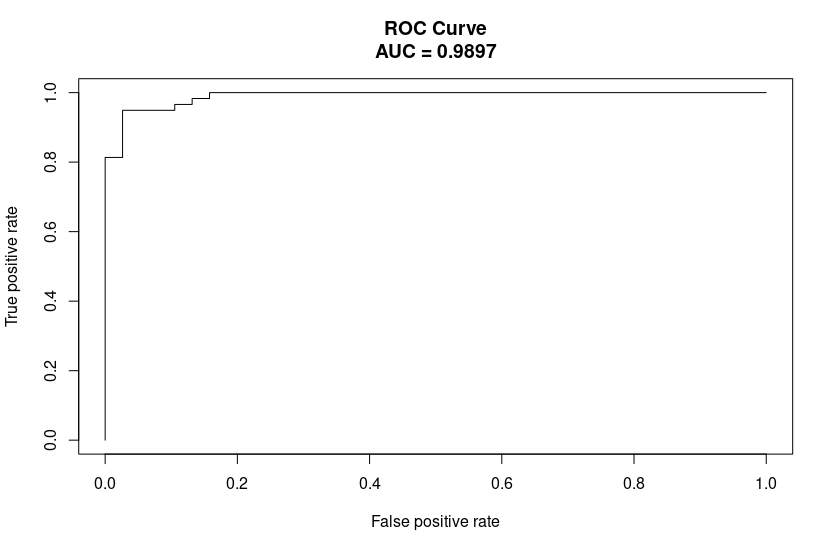
\includegraphics[scale=0.38]{roc_black_white.png}
    \caption{ROC Curve for different evaluation thresholds.}
    \label{fig:roc}
\end{figure}
%
% To start a new column (but not a new page) and help balance the last-page
% column length use \vfill\pagebreak.
% -------------------------------------------------------------------------
%\vfill
%\pagebreak
%
%\vspace{-0.5cm}
\section{RESULTS}
\label{sec:results}
In the current section, we will present the testing procedure results, both for each recording individually and for each subject in total. To keep the testing procedure unbiased, we used a variation of the Leave-one-out cross-validation. Each time we tested the algorithm results for either a 30-second recording or a subject, all of the samples belonging to the current subject were excluded from the training process.

For the individual evaluation of the recordings, the precision of the model was 96.04\%, the recall was 83.16\%, and the f-score was 89.14\%, having a total accuracy of 83.46\%. The significant difference between precision and recall was caused firstly by the imbalance of testing samples and, secondly, by the imbalance of the subjects participating in the training process.

Regarding the subjects' evaluation, we had to inspect the ideal threshold of their CAD predictions ratio. For this purpose, we created the ROC curve shown in Figure \ref{fig:roc}. The Area Under Curve (AUC) was calculated to be 0.9897\%. We decided to use 0.5 as a final threshold, meaning that subjects whose ratio of CAD to total predictions is greater than 0.5 will be characterized as having CAD; else, they will be characterized as not having CAD. With the use of this threshold, the total precision was 92.1\%, recall was 98.3\%, f-score was 95.1\%, and accuracy was 93.8\%. These results were evaluated after testing all the available recordings of each subject.
%
\section{COMPARISON AND DISCUSSION}
\label{sec:comparison}
The problem of automatic detection of CAD has been an active field of research for a long time. Various approaches have been proposed in the past two decades. Subsequently, we will refer to some of the most popular ones, compare them to our work, and comment on their differences.

In 2013, Giri et al. \cite{giri} used 15-minute ECGs and an SVM model to achieve accuracy between 85\% to 90\%. In 2017, Dolatabi et al. \cite{dolatabadi} proposed a method using one-lead 24-hour ECGs and an SVM, which reached an accuracy of 99.2\%. Also, Patidar et al. \cite{patidar} used 15-min ECGs and an LS-SVM model to achieve 99.7\% accuracy. Almost all of the previous models achieved better accuracy than our current work; however, the length of the ECG recording that these models need as input would be prohibiting for our present application. Since we try to create a tool that people can use in their everyday life, demanding long ECG recordings as input could not be practical.

As for the models that use shorter time intervals, there have been published numerous papers as well. Altan et al. \cite{altan} used 15-second ECGs and a deep belief network and achieved 98.05\% accuracy with a 10-fold validation. Acharya et al. \cite{acharya} had an accuracy of 94.95\% using 5-second ECGS, a CNN, and 10-fold validation as well, while Lih et al. \cite{lih} used 2-second ECGs, a CNN-LSTM network, and 10-fold validation and had the accuracy of 98.51\% for a 4-class problem. All of the methods mentioned above have higher accuracy and a smaller ECG duration as input. However, there is a not negligible probability that cross-validation results in an overestimation of the performance scores, since different subsets may include samples deriving from the same person, allowing the algorithms to perceive impeccable signs deriving from each heart's physiology. Thus, it can not be corroborated in real-life settings.

Finally, Tan et al. \cite{tan} used 5-second one-lead ECG recordings and a CNN and LS network. They also used a subject-specific validation which led to a 99.14\% accuracy on non-CAD subjects and 76.56\% accuracy on CAD subjects. However, the CAD dataset in that research consisted of only seven subjects.
%
\section{CONCLUSION}
\label{sec:conclusion}
The method presented in this paper proposes a non-invasive, effective, reliable, and lightweight algorithm for detecting CAD using 30-second ECG recordings. It delivers a subject-specific accuracy of 93.8\% through a blind testing procedure. Also, it is designed to accept noisy ECGs derived from smartwatches, and, moreover, it is light enough to be deployed on a regular mobile phone. All of the factors mentioned above make it suitable for an everyday application that can contribute to the early detection of CAD.
%
%\vfill\pagebreak
%
% References should be produced using the bibtex program from suitable
% BiBTeX files (here: strings, refs, manuals). The IEEEbib.bst bibliography
% style file from IEEE produces unsorted bibliography list.
% -------------------------------------------------------------------------
\bibliographystyle{IEEE}
\bibliography{strings,refs}

\end{document}
